\chapter{Lower bounds for constant depth circuits}

In 2021, Nutan Limaye, Srikanth Srinivasan and \Sebastien Tavenas~\cite{LST21} proved super-polynomial lower bounds for constant depth circuits! Not just that, but they gave a ridiculously simple proof of this fact! Needless to say, many parts of the introductory parts of various chapters alluding to lack of progress etc. has been completely blown out of the waters. Admittedly, it is a little silly to discuss fairly complicated approaches to prove lower bounds for depth-$4$ circuits etc. for the last how-many-ever chapters only to give a completely simple proof of super-polynomial lower bound for arbitrary constant depth circuits. But, well, it is what it is. 

In this chapter, we are going to see the full proof of their beautiful result and then worry about correcting the narrative in the survey later. 

\begin{theorem}[Limaye-Srinivasan-Tavenas~\cite{LST21}] Let $d,n$ such that $d = o(\log n)$. For any $\Delta > 0$, any product-depth $\Delta$ circuit computing $\IMM_{n,d}$, over any field of characteristic zero, requires size $n^{d^{-\exp(\Delta)}}$.

  For the particular case of $\Sigma\Pi\Sigma$ circuits, the lower bound is $n^{\Omega(\sqrt{d})}$. 
\end{theorem}

As we have seen in \autoref{thm:chasm-at-3}, this lower bound for $\Sigma\Pi\Sigma$ circuits is tight, up to constants in the exponent.

\paragraph{Comparing with depth-reduction results.} We have seen in \autoref{exercise:depth-reduction-prod-depth} that any polynomial sized circuit can be equivalently computed by a homogeneous product-depth $\Delta$ circuit of size at most $n^{O(d^{1/\Delta})}$. Furthermore, if we are willing to forgo homogeneity, then \autoref{thm:chasm-at-3} can be used to yield a non-homogeneous product-depth $\Delta$ circuit of size at most $n^{O(d^{1/2\Delta})}$. Therefore, the above theorem is tight for the setting of $\Delta = 1$ but not so for larger $\Delta$.

\section{Proof overview}

The proof is surprisingly extremely simple. Roughly speaking, the proof proceeds in three broad steps, many components of which were known!

\begin{enumerate}
\item\label{item:LST-step1} Convert any arbitrary product-depth $\Delta$ circuit into a homogeneous product-depth $2\Delta$ circuit computing the same polynomial.
\item\label{item:LST-step2} Convert any homogeneous product-depth $2\Delta$ circuit computing a set-multilinear polynomial into a set-multilinear product-depth $2\Delta$ circuit computing the same polynomial.
\item\label{item:LST-step3} Prove a lower bound for set-multilinear constant depth circuits. 
\end{enumerate}

Note that \autoref{lem:d3-d5} already showed a version of \autoref{item:LST-step1} to convert a non-homogeneous $\Sigma\Pi\Sigma$ circuit to a homogeneous $\Sigma\Pi\Sigma\Pi\Sigma$ circuit. Turns out, this can be generalised to larger depth as well and we'll discuss this later in the chapter.

As for \autoref{item:LST-step2}, we did see a set-multilinearisation in the context of \autoref{thm:form-to-smlform}. Turns out, the same can also be done for constant depth circuits.

As for \autoref{item:LST-step3} of proving lower bounds for set-multilinear formulas of constant depth, we even have lower bounds for multilinear formulas of arbitrary depth! However, an important point is that both the above steps are efficient only when $d \ll n$ whereas many of the multilinear and set-multilinear lower bounds required $d$ to be comparable to $n$. Nevertheless, Limaye, Srinivasan and Tavenas show how to use the same technique with a small but ingenious modification.

\section{Reducing to the set-multilinear world}

We will first see how we can transform any small-depth circuit computing a lower-degree set-multilinear polynomial into a syntactically set-multilinear small-depth circuit without too much blow-up in size. This involves two steps as mentioned above --- homogenisation and set-multilinearisation. 

\subsection{Homogenisation within small depth}

It is good to keep in mind that it is perhaps too much to expect to homogenise a non-homogeneous  arbitrary depth-$\Delta$ circuit into a homogeneous depth-$\Delta$ circuit of comparable size. An excellent counter-example to this, with respect to $\Sigma\Pi\Sigma$ circuits is the elementary symmetric polynomial. We know there are non-homogeneous $\Sigma\Pi\Sigma$ circuits of polynomial size that compute it, but any homogeneous $\Sigma\Pi\Sigma$ circuit computing it must be of exponential size (\autoref{thm:hom-depth-3-lb-esym}). 

However, if one is willing to increase the depth a little (by factor of 2), then one can indeed homogenise an arbitrary circuit with a not-too-large blow-up in size.

\begin{lemma}[Homogenisation within constant depth]\label{homogenisation-within-constant-depth}
  Let $C$ be a product-depth $\Delta$ circuit of size $s$ computing an $n$-variate degree $d$ polynomial. Then, there is a \emph{homogeneous} circuit $C'$ of product-depth $2\Delta$ and size $2^{O(\sqrt{d})} \cdot \poly(s)$ computing the same polynomial. 
\end{lemma}

We'll give the sketch of the proof here. It is instructive to go back to what we did in the case of $\Sigma\Pi\Sigma$ circuits. The crux is to try and extract the homogeneous part of a term of the form
\[
  T = (1 + \ell_1)\cdots (1 + \ell_m)
\]
where each of the $\ell_i$'s are homogeneous linear polynomials. It is clear that
\[
  \Hom_{d}(T) = \ESym_d(\ell_1,\ldots, \ell_m).
\]
Then, we can use the fact that $\ESym(z_1,\ldots, z_m)$ can be computed by a homogeneous depth-$4$ (or product-depth $2$) circuit of size at most $2^{O(\sqrt{d})}\poly(m)$ (\autoref{lem:d3-d5}). Therefore, $\Hom_d(\Sigma\Pi\Sigma)$ can be computed by a homogeneous depth-$5$ circuit of size at most $2^{O(\sqrt{d})}\poly(s)$  size.

This proves the above lemma in the setting when $\Delta = 1$. In order to generalise this to higher depth, what exactly would we need? If there is a multiplication gate $g = g_1 \times \cdots \times g_m$, and lets assume that we have managed to break each $g_i$ into its homogeneous parts $g_{i,0} + g_{i,1} + \cdots + g_{i,d}$. Therefore, we wish to extract the homogeneous part
\[
  \Hom_d(g) = \Hom_d\inparen{\prod_{i=1}^m \inparen{\sum_{j=0}^d g_{i,j}}},
\]
which seems very similar to the elementary symmetric polynomial except that it is a ``weighted'' version of it:
\[
  \WESym_{m,d}( z_{1,0}, \ldots, z_{1,d}, \ldots, z_{m,0}, \ldots, z_{m,d}) = \sum_{\substack{\sigma: [m]\rightarrow \{0,\ldots, d\}\\ \sum_{i} \sigma(i) = d}} \;\;\prod_{i=1}^m z_{i, \sigma(i)}.
\]
In words, we want all monomials obtained by picking up one homogeneous part from each block such that the total degree is exactly $d$. Very similar to Newton identities that relate the $\ESym_i$ families to the $\PSym_i$ families, there are similar relations between the weighted versions of them. This was also implicit in the work of Bera and Chakrabarti~\cite{BC15}. We'll state it here without proof but a complete proof is presented in the paper of Limaye, Srinivasan and Tavenas~\cite{LST21}.

\begin{lemmawp}[\cite{BC15}]
  The polynomial $\WESym_{m,d}$ can be computed by a homogeneous $\Sigma\Pi\Sigma\Pi$ circuit of size at most $2^{O(\sqrt{d})} \cdot \poly(m)$. 
\end{lemmawp}

Applying this at each gate of an arbitrary depth-$\Delta$ circuit yields \autoref{homogenisation-within-constant-depth}.

\subsection{Set-multilinearisation}

\begin{lemma}[Set-multilinearisation in constant depth]
  \label{lem:set-multilinearisation-constant-depth}
  Let $C$ be a homogeneous product-depth $\Delta$ circuit of size $s$ computing a set-multilinear $n$-variate degree $d$ polynomial $f$. Then, there is a \emph{set-multilinear circuit} of product-depth $\Delta$ and size $d^{O(d)} \cdot \poly(s)$ computing the same polynomial. 
\end{lemma}

This is exactly the standard set-multilinearisation operation that we used in \autoref{thm:form-to-smlform} which just needs to be inspected that the same can be done with constant depth, arbitrary fan-in circuits.

\begin{exercise}[Set-multilinearisation in constant depth]
Prove \autoref{lem:set-multilinearisation-constant-depth}. 
\end{exercise}

\section{Lower bound for set-multilinear, small-depth circuits}

Now that we have seen that any $n$-variate, degree $d$, set-multilinear polynomial that is computed by a small product-depth $\Delta$ circuit can also be computed by a set-multilinear product-depth $2\Delta$ circuit of size $d^{O(d)} \cdot \poly(s)$, it suffices to prove strong enough lower bounds for small-depth set-multilinear circuits.

\subsection{The complexity measure}

Suppose $X = X_1 \sqcup \cdots \sqcup X_d$, we will be using the familiar measure of the rank of the partial derivative matrix. We will split $d$ parts into two sets of buckets, that we'll refer to as Alice parts and Bob parts and denote them by $Y_1 \sqcup \cdots \sqcup Y_r$ and $Z_1 \sqcup \cdots \sqcup Z_{r'}$ respectively (with $r + r' = d$). For this partition of variables and this split, and for any set-multilinear polynomial $f$, we will defined the matrix $M(f)$ as follows:

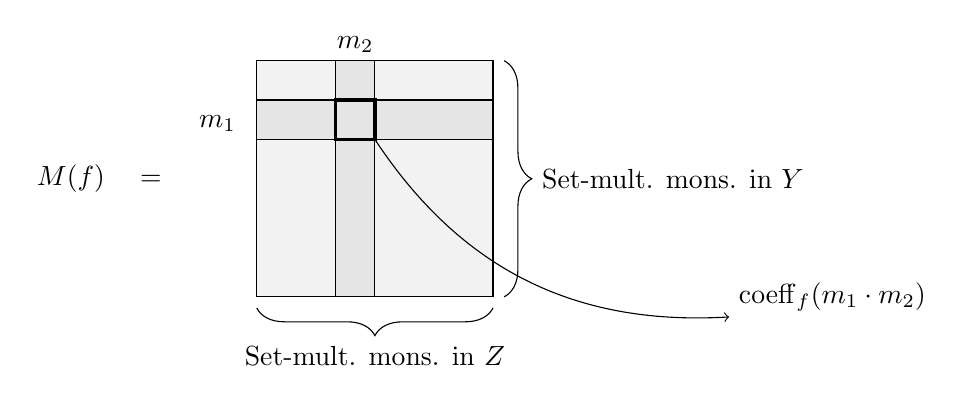
\begin{tikzpicture}
\node at (-2,1.5) {$M(f) \quad= $};
\draw[fill=black!5] (0,0) rectangle (3,3);

\draw[decorate,decoration={brace,amplitude=10pt, mirror, raise=4pt},yshift=0pt]
(3,0) -- (3,3);
\node[anchor=west] at (3.5,1.5) {Set-mult. mons. in $Y$};
\draw[decorate,decoration={brace,amplitude=10pt,mirror, raise=4pt},yshift=0pt] 
(0,0) -- (3,0);
\node[anchor=north] at (1.5,-0.5) {Set-mult. mons. in $Z$};

\draw[fill=black!10] (1,0) rectangle (1.5,3);
\node at (1.25,3.2) {$m_2$};

\draw[fill=black!10] (0,2) rectangle (3,2.5);
\node at (-0.5,2.2) {$m_1$};

\draw[very thick] (1,2) rectangle (1.5,2.5);

\node[anchor=west] at (6,0) {$\mathrm{coeff}_f(m_1 \cdot m_2)$}
edge[<-,bend left] (1.5,2);
\end{tikzpicture}

That is, this is the \emph{communication matrix} when Alice is given all variables of the Alice parts and Bob is given all variables in the Bob parts. The number of rows is $\prod \abs{Y_i}$ and the number of columns is $\prod \abs{Z_i}$. The measures used will be related to the rank of this matrix but it would be convenient to use a normalised version of this, called \emph{relative-rank} (denoted by $\relRank$).
\[
  \mu(f) := \relRank(M(f)) := \frac{\rank(M(f))}{\sqrt{\#\text{rows} \cdot \#\text{cols}}}
\]
Roughly speaking, $\relRank$ is a way of capturing the rank of the matrix and also take into account the \emph{aspect-ratio} of the matrix.

The following are a few simple observations of $\relRank$ that follows readily from the definition.
\begin{observation}[Simple properties of $\mu$]
  The following are some simple properties about the measure $\mu$:
  \begin{enumerate}
  \item \textbf{Trivial upper bound.} For any set-multilinear polynomial $f$, we have
    \[
      \mu(f) \leq \min\inbrace{\sqrt{\frac{\#\text{rows}}{\#\text{cols}}}, \sqrt{\frac{\#\text{cols}}{\#\text{rows}}}}. 
    \]
    In particular, $\mu(f) \leq 1$.
  \item \textbf{Sub-additivity.} For any set-multilinear sum\footnote{That is, $f$ and $g$ set-multilinear with respect to the same parts.} $f+g$, we have
    \[
      \mu(f+g) \leq \mu(f) + \mu(g).
    \]
  \item \textbf{Multiplicativity.} For any set-multilinear product\footnote{That is, $f$ and $g$ set-multilinear on disjoint sub-partitions.}
    \[
      \mu(f \cdot g) = \mu(f) \cdot \mu(g).
    \]
  \end{enumerate}
\end{observation}

To illustrate the key idea, we will illustrate how to get super-polynomial lower bounds for $\Sigma\Pi\Sigma$ circuits, which translates to proving good enough lower bound for set-multilinear $\Sigma\Pi\Sigma\Pi\Sigma$ circuits. 

\subsection{Lower bounds for set-multilinear depth-$5$ circuits}

Until now, we didn't really bother much about the sizes of the parts with Alice and Bob but this will be crucial! Let $k$ be a parameter that is set to $(\log_2 n)/2$ and we will assume that $k > \frac{\sqrt{d}}{2}$.

We will only consider set-multilinear polynomials of degree $d$, where each Alice part $Y_i$ has size exactly $2^{k - \frac{k}{\sqrt{d}}}$ and each Bob part $Z_j$ has size exactly $2^k$. (To avoid the use of floors and ceilings, we will assume that $k$ is divisible by $\sqrt{d}$). However, we will set up the number of Alice parts and Bob parts so that
\[
  \prod \abs{Y_i} \approx \prod \abs{Z_i}
\]
so that the matrix $M(f)$ is almost a square matrix. The imbalance between the sizes of the Alice parts and the Bob parts will be crucial in the proof.\\

The hard polynomial, for now, will be whatever $P$ makes the matrix $M(P) = I$ and hence $\mu(P) = 1$. Noticing that we can actually find an efficiently computable polynomial with $\mu(P) = 1$ is mostly an after-thought and we'll do that later. (TODO)

\subsubsection{Warm-up: Lower bounds for set-multilinear $\Sigma\Pi\Sigma$ circuits}

If $\ell$ is any set-multilinear linear polynomial, then $\ell$ must only involve a single part $X_i$. Therefore,
\[
  \mu(\ell) \leq \frac{1}{\sqrt{\abs{X_i}}}. 
\]
Hence, if $C$ is a size $s$ set-multilinear $\Sigma\Pi\Sigma$ circuit, then
\[
  \mu(C) \leq s \cdot \frac{1}{\sqrt{\abs{X_1} \cdots \abs{X_d}}}
\]

\subsubsection{The lower bound}

\begin{lemma}[Lower bound for set-multilinear depth-$5$ circuits]\label{lem:lb-sml-depth-5}
  Let $f$ be a set-multilinear polynomial with respect to the partition defined above, with $d = o(\log^2 n)$. If $f$ is computable by a size $s$, set-multilinear $\Sigma\Pi\Sigma\Pi\Sigma$ circuit, then
  \[
    \mu(f) \leq s \cdot 2^{-k \sqrt{d}/8}. 
  \]
\end{lemma}

Once we have this lemma, the lower bound is an immediate corollary.

\begin{corollarywp}
  Let $f$ be a set-multilinear polynomial with respect to the above parts with $\mu(f) = 1$. Then, any set-multilinear $\Sigma\Pi\Sigma\Pi\Sigma$ circuit computing it must have size $n^{\Omega(\sqrt{d}}$. 
\end{corollarywp}


\begin{proof}[Proof of \autoref{lem:lb-sml-depth-5}] The proof of this Lemma is embarrassingly simple. Suppose, $C = T_1 +  \cdots + T_r$ where each $T_i$ is a set-multilinear $\Pi\Sigma\Pi\Sigma$ circuit of size $s_i$, then we know that $s \leq \sum s_i$. Thanks to sub-additivity, it suffices to show that $\mu(T_i) \leq s_i \cdot 2^{-k\sqrt{d}/8}$. Hence, let us focus on one such term
  \[
    T = Q_1 \ldots Q_t
  \]
  where (reusing some variables) $T$ has size bounded by $s$ and is a set-multilinear product of set-multilinear $\Sigma\Pi\Sigma$ circuits. Without loss of generality, let $Q_1$ have the largest degree among $Q_1,\ldots, Q_t$.

  \medskip

  {\bf Case 1: $\deg(Q_1) > \sqrt{d}/2$.} In this case, $Q_1$ is a \emph{size-able} factor and hence ``the loss'' from $Q_1$ is going to be sufficient for us.
  \begin{align*}
    \mu(T) & = \mu(Q_1) \cdots \mu(Q_t) \leq \mu(Q_1)\\
           & \leq s \cdot \frac{1}{\sqrt{\abs{X_{i_1}} \cdots \abs{X_{i_{d'}}}}} \leq s \cdot 2^{-\frac{\sqrt{d}}{4} \cdot \inparen{k - \frac{k}{\sqrt{d}}}} \leq s \cdot 2^{-k\sqrt{d}/8}.
  \end{align*}

  \medskip

  {\bf Case 2: $\deg(Q_i) \leq \sqrt{d}/2$ for all $i$.} Since $\mu$ is multiplicative, we have
  \[
    \mu(T)  = \mu(Q_1) \cdots \mu(Q_t).
  \]
  We will show that $\mu(Q_i) \ll 1$ purely from the fact that $M(Q_1)$ will be far from a square matrix!

  Let us focus on one factor $Q$. Suppose this factor depends on $a$ Alice parts and $b$ Bob parts. Further, $a+b = \deg(Q) \leq \sqrt{d}/2$. Let us get a sense of the number of rows and columns in the matrix $M(Q)$.
  \begin{align*}
    \#\text{rows} & = 2^{a \cdot \inparen{k - \frac{k}{\sqrt{d}}}},\\
    \#\text{cols} & = 2^{b \cdot k},\\
    \implies \mu(Q) & \leq \min \set{\sqrt{\frac{\#\text{rows}}{\#\text{cols}}}, \sqrt{\frac{\#\text{cols}}{\#\text{rows}}}}\\
                  & = 2^{- k \cdot \abs{a\inparen{k - \frac{k}{\sqrt{d}}} - bk}} =: 2^{-k \cdot \abs{E}}
  \end{align*}
  where $E = a\inparen{1 - \frac{1}{\sqrt{d}}} - b$. The key point is that $E$ is not close to zero just for the simple reason that the fractional part of $E$ is substantial.

  \noindent
  If $a \leq b$, then $E$ is negative. Hence,
  \begin{align*}
    E & =  a\inparen{1 - \frac{1}{\sqrt{d}}} - b\\
      & \leq \frac{\deg(Q)}{2} \cdot \inparen{1 - \frac{1}{\sqrt{d}}} - \frac{\deg(Q)}{2}\\
      & = \frac{-\deg(Q)}{2\sqrt{d}}.
  \end{align*}
  If $a > b$, then $E$ is positive. There, we have
  \begin{align*}
    E & \geq \{E\} = \inbrace{1 - \frac{1}{\sqrt{d}}}\\
      & > \frac{1}{2} > \frac{\deg(Q)}{4\sqrt{d}}.
  \end{align*}
  Therefore,
  \begin{align*}
    \mu(Q) & \leq 2^{- \frac{k \cdot \deg(Q)}{4\sqrt{d}}}\\
    \implies \mu(T) & = \mu(Q_1)\cdots \mu(Q_t) \leq 2^{-\frac{k \cdot \deg(T)}{4\sqrt{d}}} = 2^{-k\sqrt{d}/4}
  \end{align*}
  And that completes the proof!  
\end{proof}


\subsection{Lower bounds for larger depth}

The lower bound for larger depth proceeds exactly along the same lines (with a few minor technical issues that need to get sorted out). Suppose we are dealing with a depth-$7$ set-multilinear circuit instead. The idea is to proceed exactly along the same lines. Say this circuit $C = T_1 + \cdots + T_r$, it suffices to focus on each summand $T_i$. Suppose such a summand $T = Q_1 \cdots Q_t$ where each $Q_i$ is now a set-multilinear depth-$5$ circuit.

{\bf Case 1: $\deg(Q_1)$ is large.} In this case, just use the upper-bound we just proved for set-multilinear depth-$5$ circuits to bound $\mu(Q_1)$ and hence $\mu(T)$.

\medskip

{\bf Case 2: All $\deg(Q_i)$'s are small.} Use the same argument to show that each $M(Q_i)$ is non-square-ish to get the upper bound on $\mu(Q_i)$ and hence $\mu(T)$.\\

The only technical hurdle is that earlier we had chosen our $k$ depending on what degree we were working with etc. but now the choice needs to be flexible. Fortunately, there is a lot of room in the choice of the parameter $k$ and this allows essentially the same argument to sail through without too much difficulty. That's basically the proof for arbitrary constant depth as well. 


\section{TODO: Subsequent results}

There were some subsequent results proved by the Limaye, Srinivasan and Tavenas that ought to be added here. Some of these include:
\begin{itemize}\itemsep0pt
\item Super-polynomial separation between depth $\Delta$ and depth $\Delta+1$
\item Super-polynomial separation between homogeneous formulas and algebraic branching programs in the non-commutative setting
\end{itemize}





%%% Local Variables: 
%%% mode: latex
%%% TeX-master: "fancymain"
%%% End: 
